\section{Higher Order Modulation}{
	\subsection{Introduction}
	{
		In this section I will go through the experiments I ran for task 2.3 the new modules I used and how I set up the parameters. \Cref{fig:2.3SimlinkModel} shows the model which I used for generating evaluating the higher order modulation functions.
		\begin{figure}
			\centering
			\includegraphics[width=\textwidth]{SimulinkModel-Task2_3}
			\caption{Shows the model used for task 2.3}
			\label{fig:2.3SimlinkModel}
		\end{figure}
	}
	\subsection{General QAM Modulator}
	{
		This converts the binary signal into a frequency signal so that it can be modified by the Rayleigh and AWGN modules. The parameters are the signal constellation which I left as the default. \Cref{fig:8QAMModulationConsetllation} shows the constellation used as you can see there are 8 points making this an 8QAM modulator.
		\begin{figure}
			\centering
			\includegraphics[width=\textwidth]{8QAMModulationConstellation}
			\caption{Shows the constellation for the QAM modulation}
			\label{fig:8QAMModulationConsetllation}
		\end{figure}
	}
	
	\subsection{General QAM Demodulator}
	{
		This converts the signal back from the frequencies to binary data. Has a constellation parameter which I have left as the default value.
	}
	\subsection{Analysis of Bit Error rates for 8-QAM}
	{
		\Cref{fig:BERBPSKVS8QAM} shows the error rates for some theoretical plots and the values for the model from task 2.2 and the new model with the QAM modulators and demodulators. As you can see QAM has worse error rates for almost all signals however this is expected as it carries more data and therefore is more susceptible to error.
		\begin{figure}
			\centering
			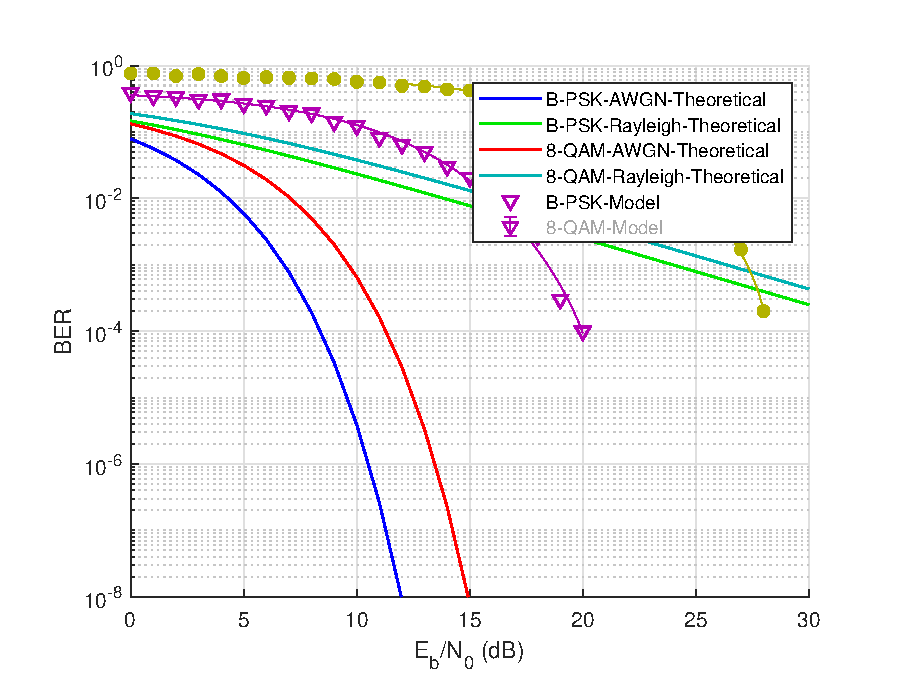
\includegraphics[width=\textwidth]{BERBPSKVS8QAM}
			\caption{Shows the BER for a number of theoretical plots and the values for my models. Note the yellow circle is actually the 8-QAM-Model}
			\label{fig:BERBPSKVS8QAM}
		\end{figure}
	}
	\subsection{Conclusion}
	{
		In this section I have gone over how I created a model which uses the QAM modulation system. Also, how the 8-QAM compares to binary psk models and why 8-QAM performs poorer than the binary psk.
	}
}